\documentclass[a4paper,12pt]{article} % тип документа

% Поля страниц
\usepackage[left=2.5cm,right=2.5cm,
    top=2cm,bottom=2cm,bindingoffset=0cm]{geometry}
    
%Пакет дял таблиц   
\usepackage{multirow} 
    
%Отступ после заголовка    
\usepackage{indentfirst}


% Рисунки
\usepackage{floatrow,graphicx,calc}
\usepackage{wrapfig}

% Создаёем новый разделитель
\DeclareFloatSeparators{mysep}{\hspace{1cm}}

% Ссылки?
\usepackage{hyperref}
\usepackage[rgb]{xcolor}
\hypersetup{				% Гиперссылки
    colorlinks=true,       	% false: ссылки в рамках
	urlcolor=blue          % на URL
}


%  Русский язык
\usepackage[T2A]{fontenc}			% кодировка
\usepackage[utf8]{inputenc}			% кодировка исходного текста
\usepackage[english,russian]{babel}	% локализация и переносы


% Математика
\usepackage{amsmath,amsfonts,amssymb,amsthm,mathtools, mathrsfs}


% Что-то 
\usepackage{wasysym}


\begin{document}
\begin{center}
	\footnotesize{ФЕДЕРАЛЬНОЕ ГОСУДАРСТВЕННОЕ АВТОНОМНОЕ ОБРАЗОВАТЕЛЬНОЕ 			УЧРЕЖДЕНИЕ ВЫСШЕГО ОБРАЗОВАНИЯ}\\
	\footnotesize{МОСКОВСКИЙ ФИЗИКО-ТЕХНИЧЕСКИЙ ИНСТИТУТ\\(НАЦИОНАЛЬНЫЙ 			ИССЛЕДОВАТЕЛЬСКИЙ УНИВЕРСИТЕТ)}\\
	\footnotesize{ФАКУЛЬТЕТ ОБЩЕЙ И ПРИКЛАДНОЙ ФИЗИКИ\\}
	\hfill \break
	\hfill\break
	\hfill\break
	\hfill \break
	\hfill \break
	\hfill \break
	\hfill \break
	\hfill \break
	\hfill \break
	\hfill \break
	\hfill \break
	\hfill \break
	\hfill \break
	\hfill \break
	\large{Лабораторная работа № Д.4.3 \\\textbf{Измерение толщины волоса}}\\
	\hfill \break
	\hfill \break
	\hfill \break
	\begin{flushright}
		Серебренников Даниил\\
		Группа Б02-826
	\end{flushright}
	\hfill \break
	\hfill \break
	\hfill \break
	\hfill \break
	\hfill \break
	\hfill \break
	\hfill \break
	\hfill \break
	\hfill \break
	\hfill \break
	\hfill \break
\end{center}
\begin{center}
	Долгопрудный, 2020 г.
\end{center}
\thispagestyle{empty}
\newpage

\textbf{Цель работы:} получить дифракционную картину на волосе и определить его толщину.

\textbf{В работе используются:} зеленая лазерная указка, волос, картон, клейкая лента, линейка, маркерная доска.

\section{Теоретическая часть}
	Случай геометрической оптики применим лишь тогда, если длина световой волны $\lambda$ много меньше характерных размеров освещаемых объектов $d$, то есть $\lambda \ll d$. При приближении размеров объектов к длине световой волны $(\lambda \sim d)$, отклонения от законов геометрической оптики, приводящие к возникновению дифракции, проявляются сильнее. Согласно принципам геометрической оптики за непрозрачным объектом должна находиться резкая геометрическая тень. В случае волновой оптики вместо резкой тени получается сложное распределение интенсивности, называемое дифракционной картиной.

	Для простоты обратимся к результатам дифракции Фраунгофера на щели. Такая дифракционная картина	состоит из центрального максимума и побочных минимумов меньшей интенсивности. Положение минимумов такой картины в приближении малых углов описывается следующим соотношением:
	\begin{equation*}
		\tag{$*$}
		\label{eq}
		m \Delta x = m \lambda \frac{L}{d},
	\end{equation*}
	где $m \in \mathbb{Z} \backslash \{0\}$ -- номер минимума, $L$ -- расстояние от щели до экрана. Отметим, что точно таким же образом описывается дифракционная картина от тонкой проволоки (волоса).

\section{Экспериментальная часть}
\subsection{Порядок выполнения работы}
	\begin{enumerate}
		\item
			 Вырежем в картоне небольшое окошко размерами примерно $2\times 4$ см. С помощью клейкой ленты закрепим в окошке натянутый волос. Разместим штатив на расстоянии $L$ от экрана.
		\item 
			 Будем светить зеленым лазером нм на волос и на экране отмечать пики дифракционной картины. В качестве экрана будем использовать белую маркерную доску.
		\item 
			 Измерим расстояния между минимумами дифракционной картины по отметкам на маркерной доске.
		\item	 
			 Для повышения точности измерений получим дифракционную картину ещё раз и повторим измерения.
		\item
			Повторим эксперимент на волосе другого человека. 
	\end{enumerate}

\newpage
\subsection{Экспериментальные данные}

	\floatsetup[table]{capposition=top}	
	\begin{table}[H]
		\caption{Некоторые измеряемые величины и их погрешность.}
		\label{table:parametr}
		\begin{tabular}{|c|c|c|c|}
			\hline
			& $L$, см & $\lambda$, нм & $\Delta x$, см \\ \hline
			Величина          & 100     & 532           & 5,0            \\ \hline
			Погрешность       & 1       & 0             & 0,2            \\ \hline
			$\varepsilon$, \% & 1       & 0             & 4              \\ \hline
		\end{tabular}
	\end{table}







	\floatsetup[table]{capposition=top}	
	\begin{table}[H]
	\caption{Результаты измерений расстояний между минимумами.}
	\label{table:exp}
	\begin{tabular}{|c|c|c|c|c|}
		\hline
		& \multicolumn{2}{c|}{Волос $D$}                         & \multicolumn{2}{c|}{Волос $G$}                                              \\ \hline
		$m$  & $\Delta x_1$, см & \multicolumn{1}{l|}{$\Delta x_2$, см} & \multicolumn{1}{l|}{$\Delta x_1$, см} & \multicolumn{1}{l|}{$\Delta x_2$, см} \\ \hline
		8  & -                & -                                     & 7,8                                   & 7,8                                   \\ \hline
		7  & 7,0              & -                                     & 7,0                                   & 6,6                                   \\ \hline
		6  & 6,1              & -                                     & 6,1                                   & 5,8                                   \\ \hline
		5  & 5,2              & 4,4                                   & 5,0                                   & 4,8                                   \\ \hline
		4  & 4,5              & 3,5                                   & 4,0                                   & 3,8                                   \\ \hline
		3  & 3,4              & 2,5                                   & 3,1                                   & 3,0                                   \\ \hline
		2  & 2,3              & 1,8                                   & 1,9                                   & 2,1                                   \\ \hline
		1  & 1,1              & 0,8                                   & 1,0                                   & 1,0                                   \\ \hline
		0  & 0,0              & 0,0                                   & 0,0                                   & 0,0                                   \\ \hline
		-1 & -0,9             & -1,0                                  & -0,9                                  & -1,0                                  \\ \hline
		-2 & -1,8             & -2,1                                  & -1,8                                  & -2,0                                  \\ \hline
		-3 & -2,8             & -2,9                                  & -2,7                                  & -2,9                                  \\ \hline
		-4 & -3,7             & -4,0                                  & -3,8                                  & -3,9                                  \\ \hline
		-5 & -4,8             & -4,9                                  & -4,8                                  & -4,9                                  \\ \hline
		-6 & -5,8             & -                                     & -5,9                                  & -5,8                                  \\ \hline
		-7 & -                & -                                     & -7,0                                  & -6,7                                  \\ \hline
		-8 & -                & -                                     & -8,0                                  & -7,7                                  \\ \hline
	\end{tabular}
	\end{table}

\newpage
\subsection{Обработка результатов}
	На основани результатов измерений, представленных в таблице~\ref{table:exp}, построим интерполяционные прямые, иллистрирующие зависмости $\Delta x = \Delta x (m)$ различных волос.
	\thisfloatsetup{floatrowsep=mysep}	
	\begin{figure}[h!]
		\begin{floatrow}
			\ffigbox[\FBwidth]{\caption{$\Delta x = \Delta x (m)$ волоса $D$.}\label{fig:Graph_1}}%
			{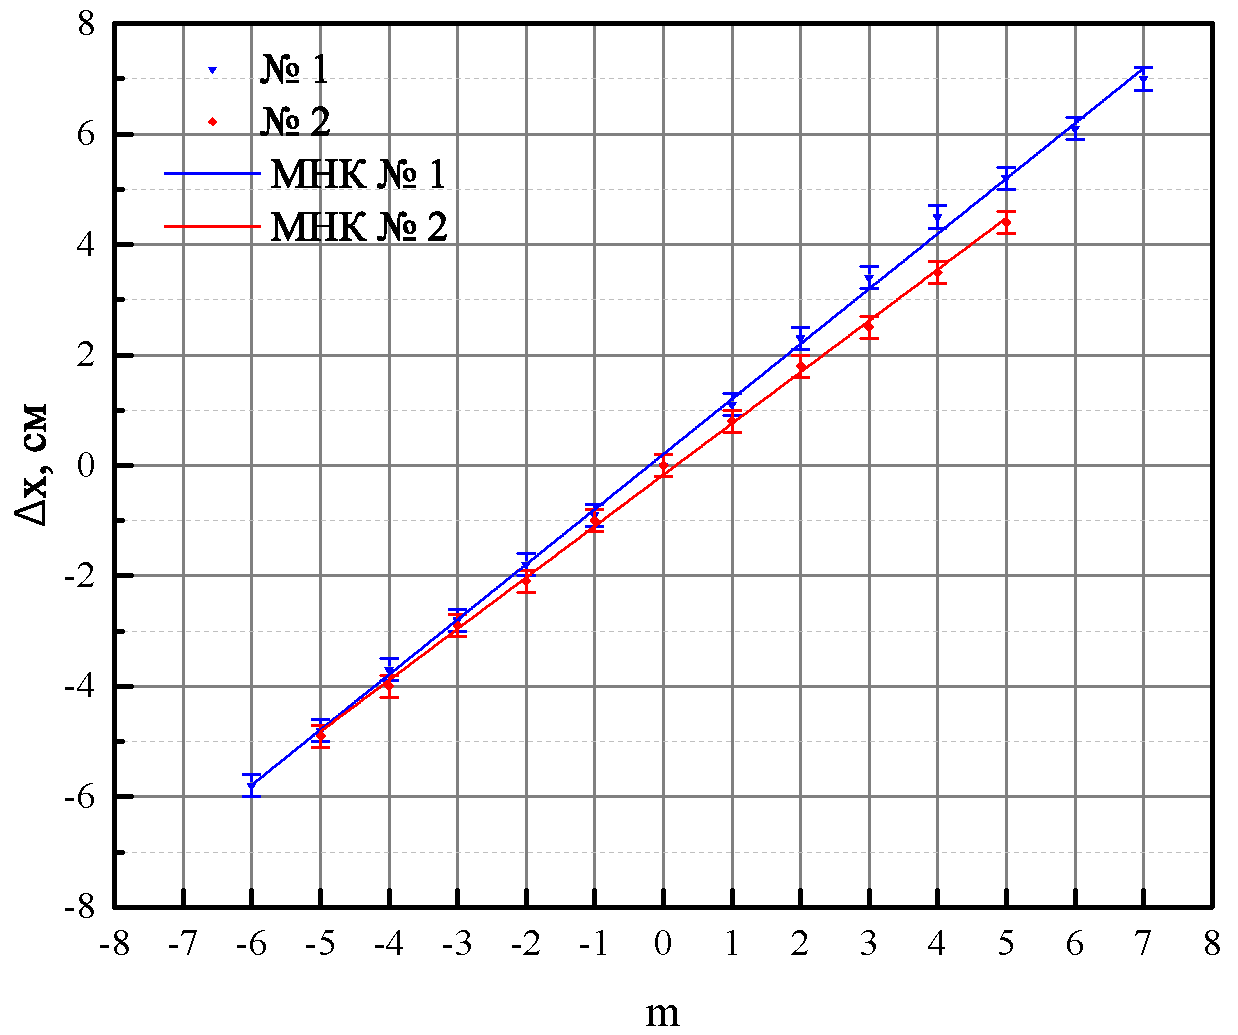
\includegraphics[width=8cm,height=7cm]{Graph1}}
			\ffigbox[\FBwidth]{\caption{$\Delta x = \Delta x (m)$ волоса $G$.}\label{fig:Graph_2}}%
			{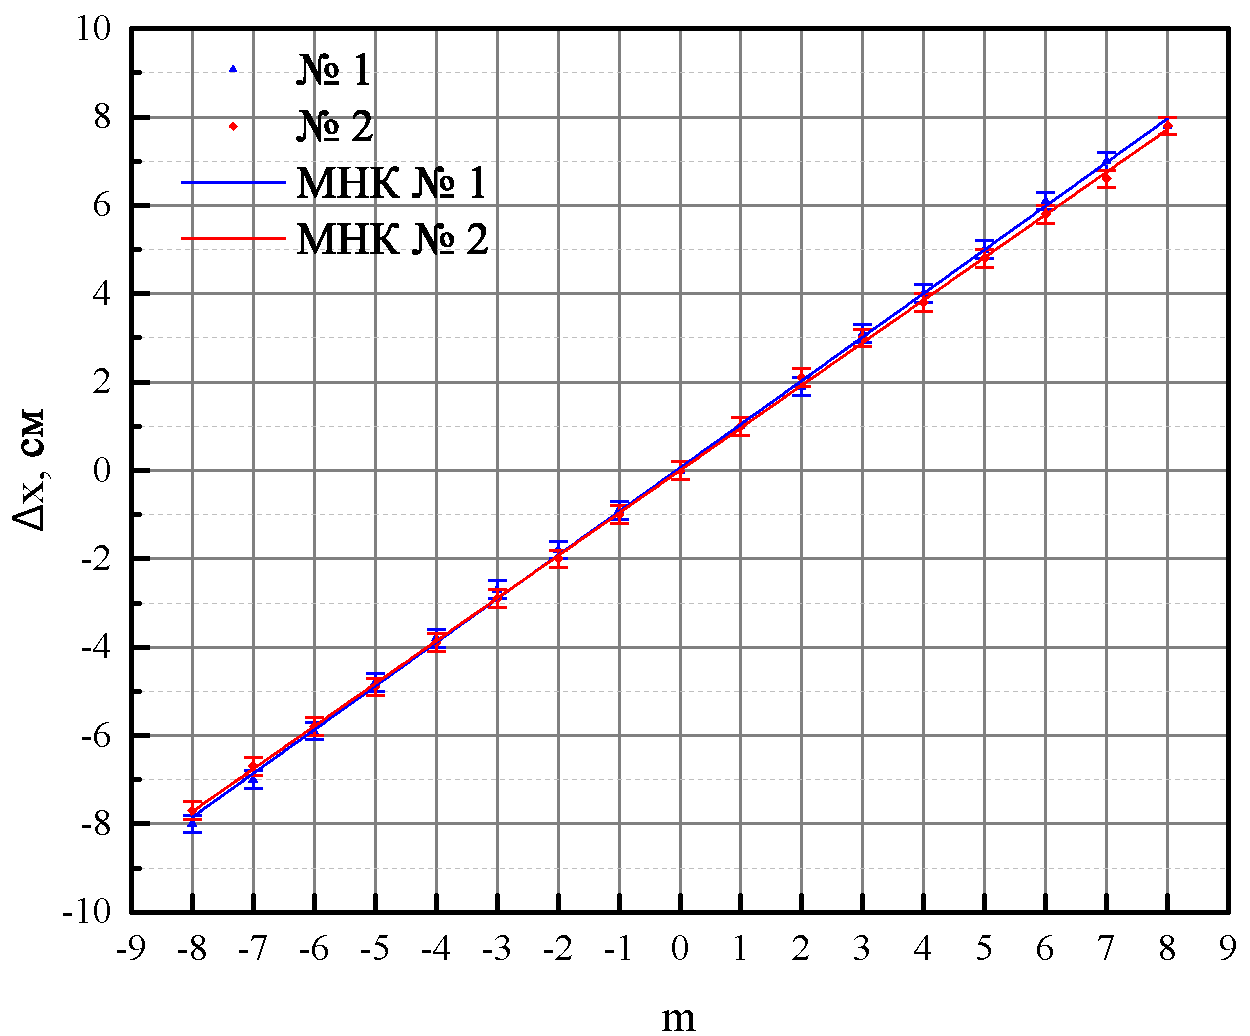
\includegraphics[width=8cm,height=7cm]{Graph2}}         
		\end{floatrow}
	\end{figure}

	В таблицах \ref{k1} и \ref{k2} представлены значения наклонов графиков, изображенных на рисунках \ref{fig:Graph_1} и \ref{fig:Graph_2} соответственно.
	
	\begin{table}[h!]
		\begin{floatrow}
			\ttabbox[\FBwidth]{\caption{Волос $D$.}\label{k1}}%
			{	\begin{tabular}{|c|c|c|}
					\hline
					& № 1   & № 2   \\ \hline
					$\Delta x / m$, см          & 0,998 & 0,930 \\ \hline
					$\sigma_{\Delta x / m}$, см & 0,010 & 0,010 \\ \hline
			\end{tabular}}
			\ttabbox[\FBwidth]{\caption{Волос $G$.}\label{k2}}%
			{\begin{tabular}{|c|c|c|}
					\hline
					& № 1   & № 2   \\ \hline
					$\Delta x / m$, см          & 0,988 & 0,965 \\ \hline
					$\sigma_{\Delta x / m}$, см & 0,005 & 0,004 \\ \hline
			\end{tabular}}        
		\end{floatrow}
	\end{table}

	Из формулы (\ref{eq}) следует, что толщина волоса есть $d_i =\lambda L (\Delta x / m)_i^{-1} $, тогда погрешность можно рассчитать следующим образом $\sigma_{d_i} = d_i \sqrt{\left(\frac{\sigma_{\Delta x / m}}{\Delta x / m}\right)_i^2 + \left(\frac{\sigma_L}{L} \right)^2}$. Рассчитанные значения усредним $d = \frac{d_1 + d_2}{2}$, причем $\sigma_d = \frac{\sigma_{d_1} + \sigma_{d_2}}{2}$. Окончательно получим:
	\[\boxed{d_D = (55,3 \ \pm \ 0,8) \ \text{мкм} }  \] \[\boxed{d_G =(54,5 \ \pm \ 0,6) \ \text{мкм} } \]
	
\section{Выводы}
	В ходе данной лабораторный работы мы наблюдали на волосе дифракционную картину, по которой определили толщину волос двух студентов ФОПФ с относительной погрешностью порядка 1,5\%. В пределах погрешноcти толщины их волос получилсь одиннаковыми.
	
	Отметим, что на экране протяженные полосы лазера чередовались не менее протяженными полосами теней. Протяженность темных участков может быть связана с тем, что глаз экспериментатора не чувствителен к низким интенсивностям света.
	
	Для повышения точности результатов можно измерить толщину большего числа волос, взятых с головы одного человека.

\end{document}	